\section{Dependence of Monte Carlo Cycles on Various Expectation Values}
\label{sec:ResultsMCcyclesExpectationValue}
When computing the expectation value of the energy and magnetization using the Ising model presented in \fxnote{secref}, the steady state will only be reached after a number of Monte Carlo cycles.
\figref{fig:ResultsMCcyclesExpectationValue1} and \ref{fig:ResultsMCcyclesExpectationValue24} show the absolute value of the expectation value of the energy and the expectation value of the magnetization for the $20\times 20$ spin case with $T = 1.0$ and $T = 2.4$, respectively. 
In each of the cases, the computation of the expectation values are made with both an ordered initial spin configuration with all spin ups and with a random initial spin configuration created by the for loop described in \fxnote{ref to section}.  
\begin{figure}[H]
\centering
\begin{minipage}{.5\textwidth}
  \centering
  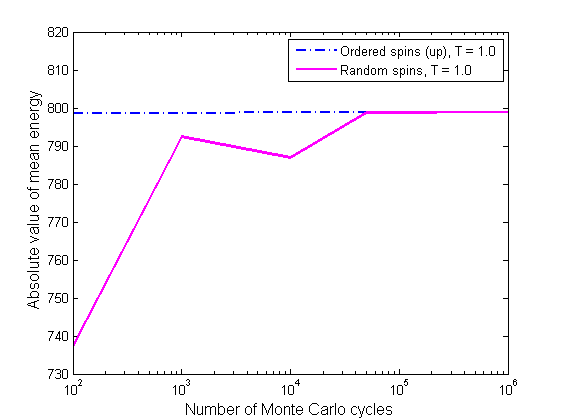
\includegraphics[width=1\linewidth]{Figures/Energy_1_0.png}
\end{minipage}%
\begin{minipage}{.5\textwidth}
  \centering
  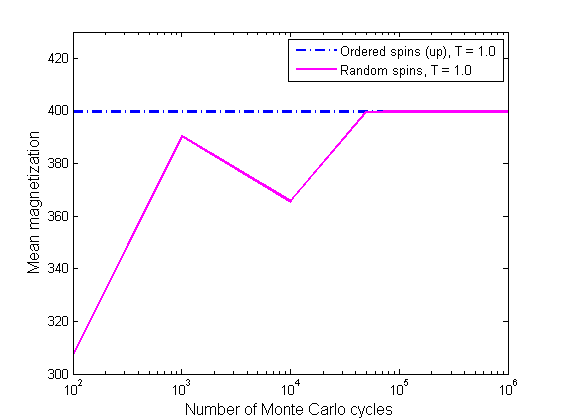
\includegraphics[width=1\linewidth]{Figures/Magnetization_1_0.png}
\end{minipage}
\caption{
The absolute value of the expectation value of the energy and the expectation value of the magnetization as functions of the number of Monte Carlo cycles for the $20\times 20$ spin case at $T = 1.0$ with ordered and random initial spin configurations.
For the case with ordered initial spin configuration, that is all spins are up, the steady state is more or less instantaneously reached since for $T = 1.0$, since the spin configuration with all spins up (or down) is the ground state with lowest energy, as for the $2\times 2$ spin case (see \figref{tab:ClosedFormSolution1}).
With a random initial spin configuration, the steady state is, however, only reached after approximately $10^5$ Monte Carlo cycles, at which the the mean of the energy stabilises at about $-799$, and the mean of the magnetization stabilises at about $400$ which was to be expected for low temperatures. 
}
\label{fig:ResultsMCcyclesExpectationValue1}
\end{figure}

\begin{figure}[H]
\centering
\begin{minipage}{.5\textwidth}
  \centering
  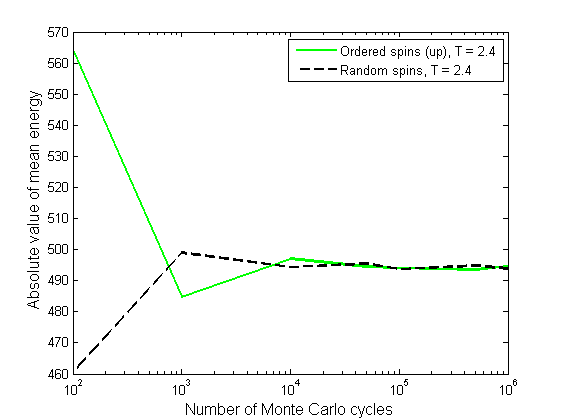
\includegraphics[width=1\linewidth]{Figures/Energy_2_4.png}
\end{minipage}%
\begin{minipage}{.5\textwidth}
  \centering
  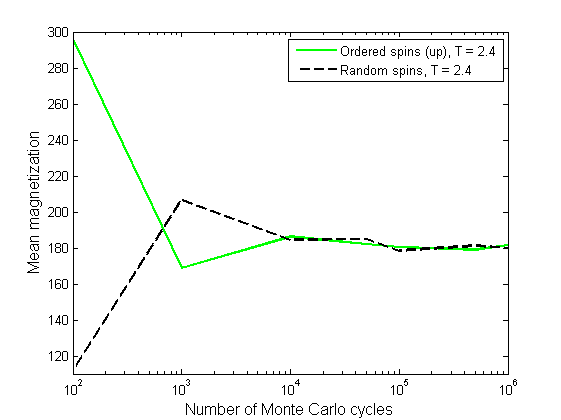
\includegraphics[width=1\linewidth]{Figures/Magnetization_2_4.png}
\end{minipage}
\caption{
The absolute value of the expectation value of the energy and the expectation value of the magnetization as functions of the number of Monte Carlo cycles for the $20\times 20$ spin case at $T = 2.4$ with ordered and random initial spin configurations.
The steady state is for both the ordered and random initial spin configuration reached after about $10^4$ Monte Carlo cycles at which the mean of the energy reaches a value of $-494$, and the mean of the magnetization reaches a value of about $180$.
}
\label{fig:ResultsMCcyclesExpectationValue24}
\end{figure}
From the graphs, it is evident that if the temperature is low, it is an advantage to have an ordered initial spin configuration with all spins up (or down), which is the spin configuration with the lowest energy.
This is due to the fact that if the temperature $T$ is low, the probability $exp(-\Delta T/T)$ of jumbing to a state with higher energy, which is equivalent to accepting a spin flip that causes a positive energy change $\Delta E$, will be low.
However, when the temperature increases to e.g. $T = 2.4$, the probability of accepting a flip that causes an increase in energy is greater, and hence a random initial spin configuration can be just as good as an ordered initial spin configuration.  